\documentclass[11pt,a4paper]{report}

% =============================================================================
% PACKAGES ET CONFIGURATION LINGUISTIQUE & TYPOGRAPHIQUE
% =============================================================================
\usepackage[utf8]{inputenc}
\usepackage[T1]{fontenc}
\usepackage[french]{babel}
\usepackage{lmodern}
\usepackage{geometry}
\geometry{
    a4paper,
    left=25mm,
    right=25mm,
    top=25mm,
    bottom=25mm
}

\usepackage{graphicx}
\usepackage{xcolor}
\definecolor{emsigreen}{RGB}{5, 150, 105}
\definecolor{emsidark}{RGB}{17, 24, 39}
\definecolor{grayborder}{RGB}{209, 213, 219}
\definecolor{tableheader}{RGB}{243, 244, 246}

\usepackage{booktabs}
\usepackage{tabularx}
\usepackage{colortbl}
\usepackage{array}
\usepackage{titlesec}
\usepackage{enumitem}
\usepackage{fancyhdr}
\usepackage[
    colorlinks=true,
    linkcolor=emsigreen,
    urlcolor=emsigreen,
    citecolor=emsigreen,
    pdfauthor={Équipe D2SI EMSI Marrakech},
    pdftitle={Cahier des charges EMSI Campus ERP}
]{hyperref}

% Configuration des titres de chapitres et sections (Modèle EMSI PFA)
\titleformat{\chapter}[hang]
  {\normalfont\LARGE\bfseries\color{emsigreen}}{\thechapter\quad}{0pt}{}
\titlespacing*{\chapter}{0pt}{-10pt}{18pt}

\titleformat{\section}
  {\normalfont\Large\bfseries\color{emsidark}}{\thesection\quad}{0pt}{}
\titlespacing*{\section}{0pt}{14pt}{6pt}

\titleformat{\subsection}
  {\normalfont\large\bfseries\color{emsidark}}{\thesubsection\quad}{0pt}{}
\titlespacing*{\subsection}{0pt}{10pt}{4pt}

% Configuration des en-têtes et pieds de page
\pagestyle{fancy}
\fancyhf{}
\fancyhead[L]{\small\color{gray} EMSI Campus ERP — Cahier des Charges}
\fancyhead[R]{\small\color{gray} Filière D2SI / IIR}
\fancyfoot[C]{\thepage}
\renewcommand{\headrulewidth}{0.4pt}
\renewcommand{\footrulewidth}{0pt}

\begin{document}

% =============================================================================
% PAGE DE GARDE OFFICIELLE (EXACTE AU MODÈLE DU PFA FOURNI)
% =============================================================================
\begin{titlepage}
    \thispagestyle{empty}
    \begin{center}
        
        % En-tête Logos : Logo EMSI à gauche et Nom du Projet à droite
        \begin{tabular*}{\textwidth}{@{\extracolsep{\fill}} lr}
            
\includegraphics[height=1.8cm]{assets/emsi_logo.png} &
            \parbox{6.5cm}{\raggedleft \textbf{\Large\color{emsigreen} EMSI Campus ERP}\\\small\color{gray} Projet PFA 2025--2026}
        \end{tabular*}
        
        \vspace{1.2cm}
        
        {\large\bfseries\color{emsidark} ÉCOLE MAROCAINE DES SCIENCES DE L'INGÉNIEUR}\\[0.2cm]
        {\small\bfseries FILIÈRE : INGÉNIERIE INFORMATIQUE ET RÉSEAUX (IIR)}\\[0.1cm]
        {\small\bfseries\color{emsigreen} OPTION : DÉVELOPPEMENT DIGITAL \& SYSTÈMES D'INFORMATION (D2SI)}
        
        \vspace{0.6cm}
        \textcolor{grayborder}{\rule{\textwidth}{1.5pt}}
        \vspace{0.6cm}
        
        {\LARGE\bfseries\color{emsidark} CAHIER DES CHARGES DE PROJET}\\[0.4cm]
        {\Large\bfseries\color{emsigreen} Système Intégré de Gestion Académique, Logistique et Planification Multi-Sites Assistée par IA (EMSI Campus ERP)}\\[0.3cm]
        {\small\itshape\color{gray} Automatisation des emplois du temps (Gueliz \& Targa), saisie directe des notes (Zéro Excel), émargement QR rotatif et matching intelligent des soutenances PFE}
        
        \vspace{0.6cm}
        \textcolor{grayborder}{\rule{\textwidth}{1.5pt}}
        \vspace{1.5cm}
        
        % Tableau Réalisateurs et Encadrants
        \begin{tabular*}{\textwidth}{@{\extracolsep{\fill}} p{8cm} p{7.5cm}}
            \textbf{Réalisé par l'équipe d'ingénieurs :} & \textbf{Encadré par :} \\[0.3cm]
            $\bullet$ Élève-Ingénieur 1 (Lead Architecture \& DB) & $\bullet$ \textbf{Pr. ZGANDRI} (Encadrante Académique) \\[0.15cm]
            $\bullet$ Élève-Ingénieur 2 (Lead Frontend Web) & \textbf{Présenté devant le jury composé de :} \\
            $\bullet$ Élève-Ingénieur 3 (Lead Mobile Flutter) & $\bullet$ \textbf{Pr. AIT OUNEJJAR Lahoussaine} (Président Jury) \\[0.3cm]
            $\bullet$ Élève-Ingénieur 4 (Backend Core \& Règles) & \textbf{Année Universitaire :} 2025--2026 \\
            $\bullet$ Élève-Ingénieur 5 (Moteur OR-Tools \& IA) & \textbf{Centre :} EMSI Marrakech (Gueliz \& Targa) \\
            $\bullet$ Élève-Ingénieur 6 (DevOps \& Sécurité CNDP) & \\
        \end{tabular*}
        
    \end{center}
\end{titlepage}

\pagenumbering{roman}

% =============================================================================
% PAGE i : PAGE DES SIGNATURES OFFICIELLES
% =============================================================================
\chapter*{Page des Signatures Officielles}
\addcontentsline{toc}{chapter}{Page des Signatures Officielles}

Le présent cahier des charges formalise l'engagement mutuel et contractuel entre l'équipe de réalisation et le corps professoral encadrant pour la conception et le développement de la plateforme logicielle \textbf{EMSI Campus ERP}.

\vspace{0.8cm}

\begin{table}[h!]
\centering
\renewcommand{\arraystretch}{1.6}
\begin{tabularx}{\textwidth}{|X|p{7cm}|}
\hline
\rowcolor{tableheader}
\textbf{Intervenant \& Rôle dans le Projet} & \textbf{Signature et Émargement} \\
\hline
Élève-Ingénieur 1 (Chef de Projet \& Architecte) & Signature : \dotfill \\
\hline
Élève-Ingénieur 2 (Lead Frontend Web Next.js) & Signature : \dotfill \\
\hline
Élève-Ingénieur 3 (Lead Mobile Flutter) & Signature : \dotfill \\
\hline
Élève-Ingénieur 4 (Lead Backend Spring Boot) & Signature : \dotfill \\
\hline
Élève-Ingénieur 5 (Spécialiste OR-Tools \& IA) & Signature : \dotfill \\
\hline
Élève-Ingénieur 6 (DevOps, QA \& Sécurité CNDP) & Signature : \dotfill \\
\hline
\rowcolor{tableheader}
\textbf{Pr. ZGANDRI} (Encadrante Académique) & Signature : \dotfill \\
\hline
\rowcolor{tableheader}
\textbf{Pr. AIT OUNEJJAR Lahoussaine} (Président de Jury) & Signature : \dotfill \\
\hline
\end{tabularx}
\end{table}

\vspace{1.2cm}
\begin{flushright}
    \textbf{Fait à Marrakech, le 16 octobre 2026}
\end{flushright}

\clearpage

% =============================================================================
% PAGE ii : LISTE DES ABREVIATIONS
% =============================================================================
\chapter*{Liste des Abréviations}
\addcontentsline{toc}{chapter}{Liste des Abréviations}

\begin{table}[h!]
\centering
\renewcommand{\arraystretch}{1.4}
\begin{tabularx}{\textwidth}{p{3.5cm} X}
\toprule
\textbf{Acronyme} & \textbf{Définition \& Signification Complète} \\
\midrule
\textbf{ERP} & Enterprise Resource Planning (Progiciel de Gestion Intégré) \\
\textbf{EMSI} & École Marocaine des Sciences de l'Ingénieur \\
\textbf{D2SI} & Développement Digital et Systèmes d'Information \\
\textbf{IIR} & Ingénierie Informatique et Réseaux \\
\textbf{EDT} & Emploi du Temps \\
\textbf{OR-Tools} & Google Operations Research Tools (Solveur Combinatoire CP-SAT) \\
\textbf{LLM} & Large Language Model (Modèle de Langage pour l'IA) \\
\textbf{JWT} & JSON Web Token (Jeton d'authentification chiffré) \\
\textbf{RBAC} & Role-Based Access Control (Contrôle d'accès basé sur les rôles) \\
\textbf{CNDP} & Commission Nationale de contrôle de la protection des Données (Loi 09-08) \\
\textbf{SLA} & Service Level Agreement (Contrat de Niveau de Service) \\
\textbf{TDD} & Test-Driven Development (Développement Piloté par les Tests) \\
\textbf{PFE / PFA} & Projet de Fin d'Études / Projet de Fin d'Année \\
\textbf{FCM} & Firebase Cloud Messaging (Notifications Push Mobiles) \\
\bottomrule
\end{tabularx}
\end{table}

\clearpage

% =============================================================================
% PAGES iii ET iv : TABLE DES FIGURES ET LISTE DES TABLEAUX
% =============================================================================
\listoffigures
\addcontentsline{toc}{chapter}{\listfigurename}

\vspace{1cm}

\listoftables
\addcontentsline{toc}{chapter}{\listtablename}

\clearpage

% =============================================================================
% PAGES v ET vi : TABLE DES MATIERES
% =============================================================================
\tableofcontents

\clearpage
\pagenumbering{arabic}

% =============================================================================
% 1. INTRODUCTION
% =============================================================================
\chapter{Introduction}

\section{Contexte et présentation du projet}
Dans les institutions d'enseignement supérieur d'ingénierie, la gestion intégrée des activités académiques, logistiques et administratives représente un défi organisationnel majeur. L'augmentation continue du nombre d'étudiants et l'expansion multi-sites entraînent une complexification des emplois du temps, une saturation des laboratoires informatiques spécialisés, ainsi que des difficultés de suivi de l'assiduité et des évaluations.

\begin{figure}[h!]
    \centering
    
\includegraphics[width=0.45\textwidth]{assets/emsi_logo.png}
    \caption{Logo officiel de l'application EMSI Campus ERP}
    \label{fig:logo_emsi}
\end{figure}

Les systèmes traditionnels de gestion reposent généralement sur des saisies manuelles ou sur des outils bureautiques dispersés (tableurs Excel, échanges d'emails non sécurisés), incapables d'assurer une supervision en temps réel et une exploitation optimale des ressources. Le projet \textbf{EMSI Campus ERP} propose la conception et le déploiement d'une plateforme unifiée combinant applications Web réactives, applications mobiles natives, programmation sous contraintes et intelligence artificielle locale souveraine.

\section{Problématique}
À l'EMSI Marrakech en particulier, la coexistence de deux campus géographiquement distants (Gueliz et Targa) génère des contraintes de déplacement majeures pour les enseignants permanents et vacataires. L'absence de temps de battement calculé automatiquement provoque des retards chroniques et une sous-exploitation des salles. 

Parallèlement, la saisie des notes d'examens sur des fichiers Excel isolés engendre des risques élevés d'erreurs de calcul, l'absence de traçabilité des modifications et une lourdeur extrême lors des délibérations semestrielles. Enfin, l'oubli fréquent de la consignation du cahier de texte à la fin des séances et l'affectation manuelle et non homogène des jurys de PFE nuisent à l'efficacité académique.

\section{Objectifs du projet}
Les objectifs spécifiques et mesurables du projet sont :
\begin{itemize}[leftmargin=1.5cm]
    \item Garantir une planification sans aucun conflit physique avec respect d'un délai minimal de 45 minutes de transit entre toute séance à Gueliz et à Targa.
    \item Garantir un temps de réponse inférieur à 2 secondes pour toute requête utilisateur sur le Web et sur mobile.
    \item Permettre la gestion simultanée d'au moins 1 000 connexions utilisateurs sans dégradation notable des performances.
    \item Supprimer à 100 \% l'usage des fichiers Excel pour la saisie des notes et automatiser l'application des seuils éliminatoires ($< 7.00/20.00$).
    \item Fournir un tableau de bord interactif pour la supervision en temps réel de l'état d'avancement des cours et des délibérations officielles.
\end{itemize}

\section{Portée du projet}
Le projet englobe le portail Web administratif (React/Next.js 14), l'application mobile native (Flutter 3.x), l'API backend d'entreprise (Spring Boot 3.3 / Java 21), le solveur sous contraintes (Google OR-Tools CP-SAT) et le serveur d'IA locale (Ollama Llama 3.2). Sont explicitement exclus du périmètre initial : le paiement direct par carte bancaire en ligne (maintenu par virement/chèque avec reçu) et la gestion de la flotte de transport.

% =============================================================================
% 2. PARTIES PRENANTES ET ACTEURS
% =============================================================================
\chapter{Parties prenantes et acteurs}

\section{Parties prenantes}
Les principales parties prenantes comprennent la Direction Générale et Pédagogique de l'EMSI, les responsables de filières (D2SI, IIR, 2IA, Génie Industriel, Génie Civil), les enseignants (permanents et vacataires), les élèves-ingénieurs, les services administratifs et financiers.

\section{Acteurs du système}
Le contrôle d'accès repose sur le principe du moindre privilège (RBAC) avec 7 rôles distincts :
\begin{itemize}[leftmargin=1.5cm]
    \item \textbf{Super Administrateur :} Gestion globale, création des comptes de direction et paramétrage multi-tenant.
    \item \textbf{Responsable de Filière :} Gestion des maquettes pédagogiques, validation des EDT et jurys de délibération.
    \item \textbf{Responsable de Planification :} Définition des contraintes matérielles des salles et exécution du solveur OR-Tools.
    \item \textbf{Enseignant :} Consultation EDT, émargement QR rotatif, remplissage du cahier de texte mobile, saisie directe des notes.
    \item \textbf{Étudiant :} Consultation emploi du temps, scan de présence, consultation des notes et téléchargement des templates PFE.
    \item \textbf{Service Scolarité :} Gestion des inscriptions, validation des justificatifs d'absence, délivrance des attestations.
    \item \textbf{Service Financier :} Suivi des encaissements, reliquats de scolarité et activation du verrou administratif.
\end{itemize}

% =============================================================================
% 3. BESOINS FONCTIONNELS
% =============================================================================
\chapter{Besoins fonctionnels}

\section{Matrice Acteurs et Fonctionnalités}
Le tableau \ref{tab:acteurs_fonctions} synthétise les interactions entre les profils utilisateurs et les fonctionnalités de la plateforme.

\begin{table}[h!]
\centering
\small
\renewcommand{\arraystretch}{1.3}
\begin{tabularx}{\textwidth}{|X|c|c|c|c|c|c|c|}
\hline
\rowcolor{tableheader}
\textbf{Fonctionnalités} & \textbf{Admin} & \textbf{Resp. Fil.} & \textbf{Planif.} & \textbf{Prof} & \textbf{Étudiant} & \textbf{Scolarité} & \textbf{Finance} \\
\hline
Gestion des comptes et rôles & \textbf{X} & & & & & & \\
\hline
Configuration filières / modules & \textbf{X} & \textbf{X} & & & & & \\
\hline
Génération automatique EDT & & \textbf{X} & \textbf{X} & & & & \\
\hline
Consultation de l'emploi du temps & & \textbf{X} & \textbf{X} & \textbf{X} & \textbf{X} & & \\
\hline
Émargement par QR Code 15s & & & & \textbf{X} & \textbf{X} & & \\
\hline
Cahier de texte via Push Mobile & & \textbf{X} & & \textbf{X} & & & \\
\hline
Saisie des notes (Zéro Excel) & & \textbf{X} & & \textbf{X} & & & \\
\hline
Calcul Délibérations \& PV officiel & & \textbf{X} & & & & \textbf{X} & \\
\hline
Matching IA des jurys PFE & & \textbf{X} & & \textbf{X} & \textbf{X} & & \\
\hline
Scolarité \& Verrou administratif & & & & & & \textbf{X} & \textbf{X} \\
\hline
\end{tabularx}
\caption{Matrice croisée Acteurs / Fonctionnalités du système EMSI Campus ERP}
\label{tab:acteurs_fonctions}
\end{table}

\section{Planification multi-sites et contrainte de transit}
Le moteur d'optimisation combinatoire intègre une contrainte spatio-temporelle rigide : si une séance dispensée pour un groupe ou par un enseignant se termine sur le campus de Gueliz et que la suivante est programmée à Targa, un délai incompressible de \textbf{45 minutes} est automatiquement injecté par le solveur. Les salles de travaux pratiques sont allouées en fonction de l'inventaire effectif des ordinateurs et de la présence de cartes graphiques GPU pour les cours d'IA et de calcul intensif.

\section{Émargement par QR Code rotatif dynamique}
Pour éliminer les feuilles de présence papier et prévenir la fraude par partage de captures d'écran, le système projette un QR code dynamique renouvelé toutes les \textbf{15 secondes}. L'application mobile de l'étudiant vérifie la validité du jeton cryptographique et valide la présence en moins d'une seconde.

\section{Clôture de séance et notification push mobile}
À la fin officielle de chaque séance, le backend envoie automatiquement une notification push haute priorité sur le smartphone de l'enseignant. Celui-ci dispose d'une interface mobile ergonomique pour renseigner en 30 secondes le chapitre traité, les travaux dirigés effectués et les devoirs assignés.

\section{Saisie directe des notes (Zéro Excel) et Délibérations}
Les enseignants saisissent les évaluations directement sur l'interface Web sécurisée avec contrôles de bornes (0.00 à 20.00). Le système applique automatiquement la règle éliminatoire : toute note à l'examen final strictement inférieure à \textbf{7.00/20.00} entraîne l'ajournement immédiat du module. Les procès-verbaux de délibération sont générés en PDF avec signature numérique infalsifiable.

\section{Soutenances PFE et matching intelligent par IA}
Les élèves-ingénieurs téléchargent directement sur la plateforme les gabarits officiels de l'EMSI (modèle Word, classe LaTeX et présentation PowerPoint). Lors de la soumission du rapport, le modèle de langage local Ollama (Llama 3.2) analyse le résumé technique, extrait les stacks technologiques et associe un jury expert du même domaine de compétences.

\begin{figure}[h!]
    \centering
    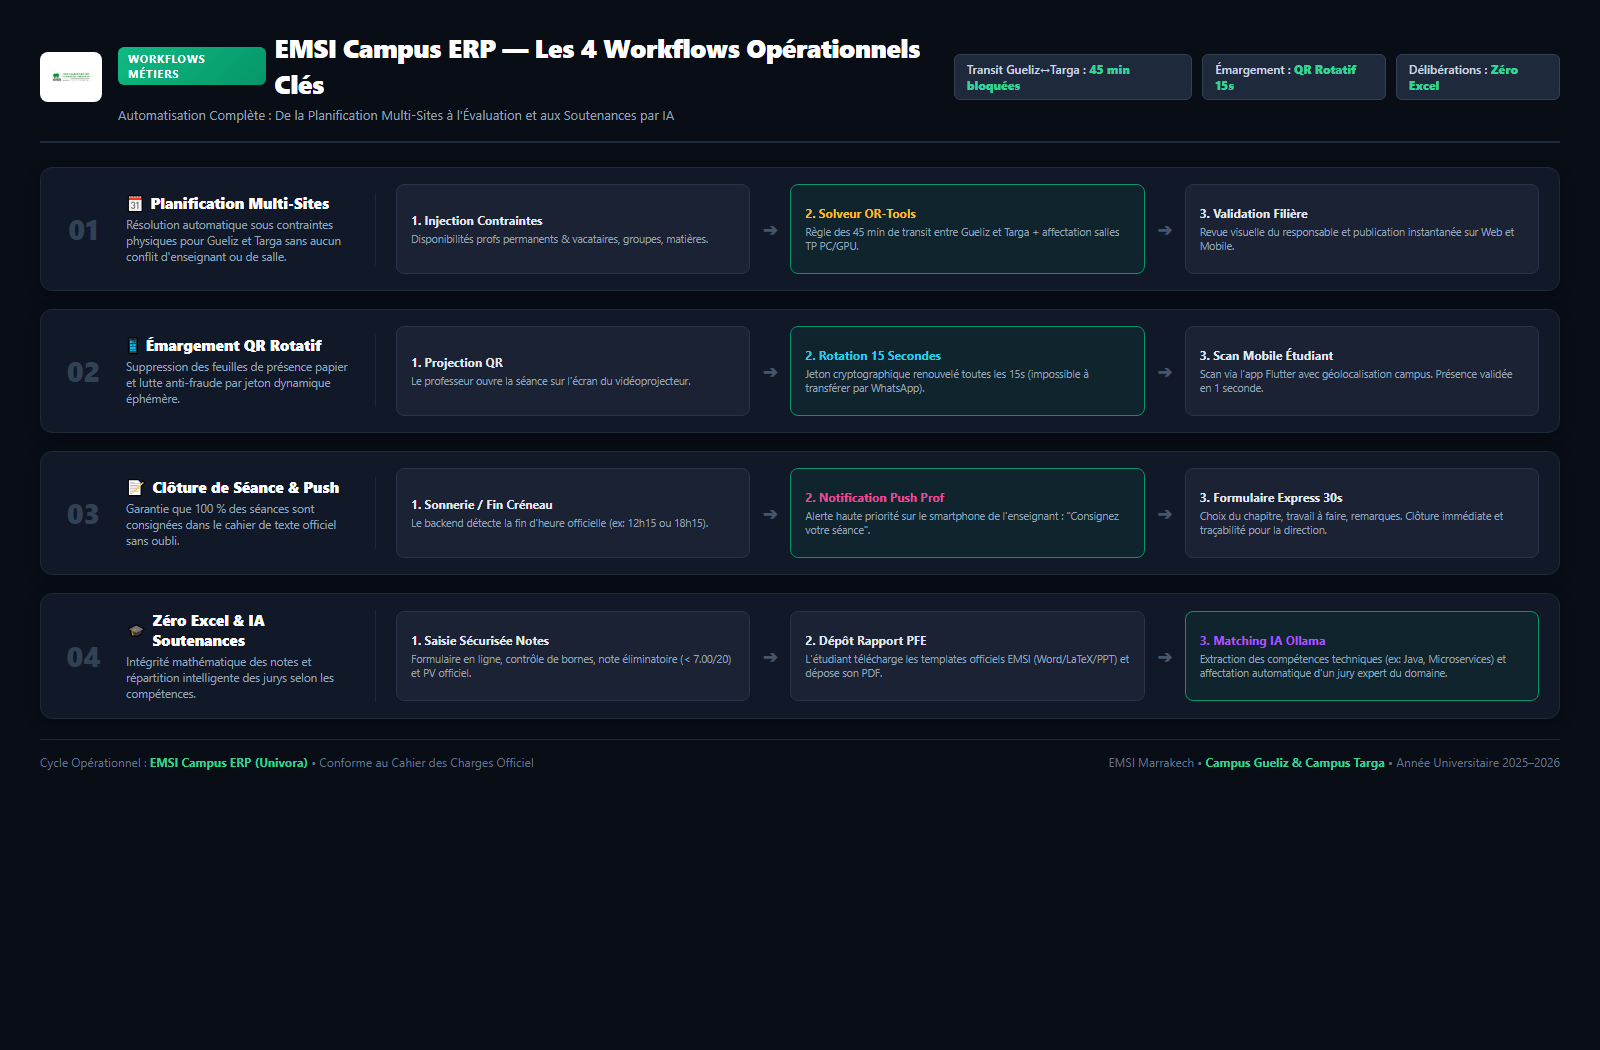
\includegraphics[width=0.95\textwidth]{assets/diagram_4_workflow_seance_soutenance.png}
    \caption{Schéma fonctionnel et workflows détaillés du système intégré}
    \label{fig:workflows_seance}
\end{figure}

% =============================================================================
% 4. BESOINS NON FONCTIONNELS
% =============================================================================
\chapter{Besoins non fonctionnels}

\begin{itemize}[leftmargin=1.5cm]
    \item \textbf{Performance :} Temps de réponse inférieur à 2 secondes pour les requêtes transactionnelles, et inférieur à 300 millisecondes pour la consultation de l'emploi du temps via Redis. Résolution complète de l'EDT par OR-Tools en moins de 3 minutes.
    \item \textbf{Disponibilité et Fiabilité :} Taux de disponibilité annuel supérieur à 99.5 \%, conteneurisation Docker et redémarrage automatique en cas d'anomalie.
    \item \textbf{Sécurité :} Authentification stateless par jetons JWT, hachage des mots de passe par algorithme BCrypt, communications chiffrées HTTPS sous TLS 1.3, isolation multi-tenant stricte par colonne \texttt{tenant\_id}.
    \item \textbf{Accessibilité :} Compatibilité Web responsive (Chrome, Edge, Firefox, Safari) et mobile native (Android API 26+, iOS 15+).
\end{itemize}

% =============================================================================
% 5. ARCHITECTURE TECHNIQUE
% =============================================================================
\chapter{Architecture technique}

\begin{figure}[h!]
    \centering
    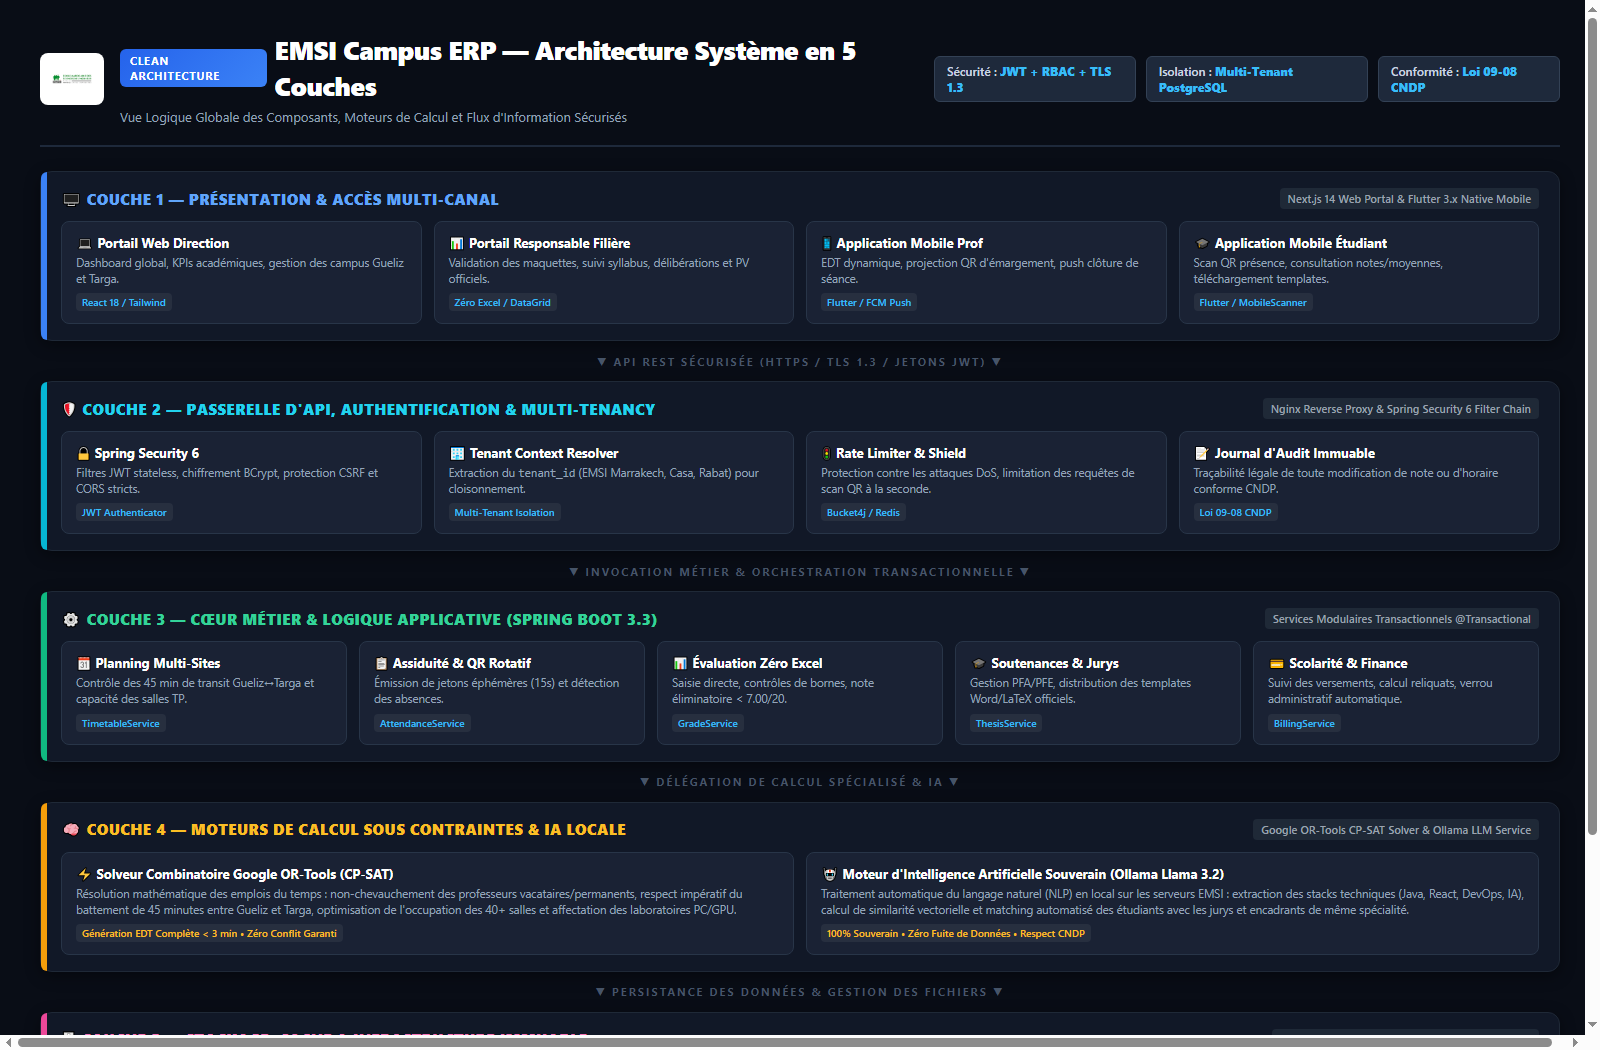
\includegraphics[width=0.95\textwidth]{assets/diagram_2_system_architecture_5layers.png}
    \caption{Architecture système globale en 5 couches logiques}
    \label{fig:archi_5layers}
\end{figure}

L'architecture du système repose sur un découpage en 5 couches logiques :
\begin{enumerate}[leftmargin=1.5cm]
    \item \textbf{Couche Présentation :} Portail Web d'administration développé sous Next.js 14 / React 18 avec Tailwind CSS, et Application Mobile native développée sous Flutter 3.x (Dart) avec Riverpod.
    \item \textbf{Couche Sécurité et Passerelle :} Reverse Proxy Nginx, Spring Security 6 avec filtres JWT stateless et contrôle de débit contre les attaques par déni de service.
    \item \textbf{Couche Métier :} Services applicatifs Spring Boot 3.3 (Java 21 LTS) orchestrant les transactions avec intégrité ACID.
    \item \textbf{Couche Calcul et IA :} Solveur de programmation par contraintes Google OR-Tools (CP-SAT) et serveur d'intelligence artificielle locale Ollama.
    \item \textbf{Couche Données et Stockage :} Système de gestion de base de données PostgreSQL 16 (40 tables Flyway), cache mémoire Redis 7 et stockage objet MinIO S3 pour les rapports et conventions.
\end{enumerate}

\begin{figure}[h!]
    \centering
    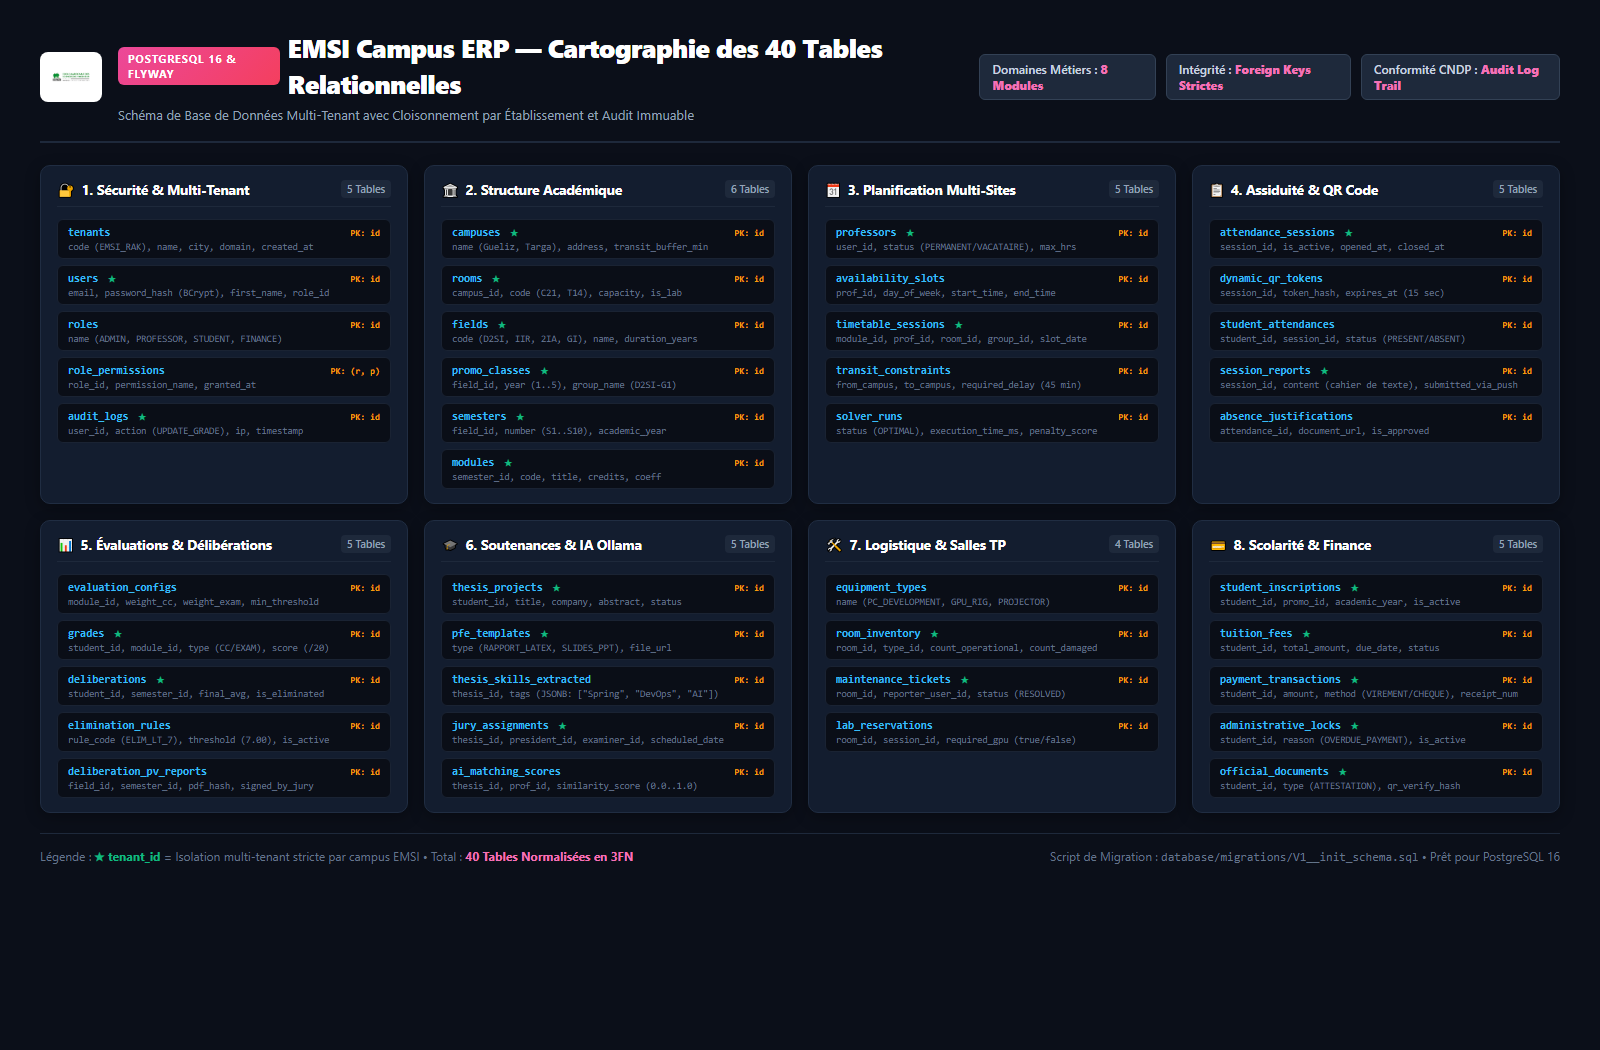
\includegraphics[width=0.95\textwidth]{assets/diagram_3_database_erd_modules.png}
    \caption{Modèle conceptuel et relations des données clés (40 tables)}
    \label{fig:erd_tables}
\end{figure}

% =============================================================================
% 6. PLANIFICATION DU PROJET
% =============================================================================
\chapter{Planification du projet (Agile Scrum + XP)}

Le développement est échelonné sur 10 semaines selon une approche hybride Scrum + Extreme Programming (XP) :
\begin{itemize}[leftmargin=1.5cm]
    \item \textbf{Sprint 0 (Semaines 1--2) :} Initialisation du monorepo, Docker Compose, migrations Flyway V1 (40 tables) et chaîne d'intégration continue CI/CD.
    \item \textbf{Sprint 1 (Semaines 3--4) :} Authentification JWT, gestion des campus Gueliz et Targa, modélisation du solveur OR-Tools avec la règle des 45 minutes de transit.
    \item \textbf{Sprint 2 (Semaines 5--6) :} Émargement QR rotatif (15s) et notification push mobile pour le remplissage obligatoire du cahier de texte.
    \item \textbf{Sprint 3 (Semaines 7--8) :} Module Zéro Excel, calculs des délibérations avec note éliminatoire ($< 7/20$), et verrou administratif de scolarité.
    \item \textbf{Sprint 4 (Semaines 9--10) :} Dépôt des PFE, matching IA des jurys avec Ollama, tests E2E automatisés et recette fonctionnelle.
\end{itemize}

\vspace{0.5cm}
\noindent\textbf{Clause de pénalité de retard :} Tout retard de livraison imputable à l'équipe de réalisation entraîne l'application d'une pénalité contractuelle de 1 \% par jour ouvré de retard, plafonnée à 10 \% de la valeur contractuelle du projet.

% =============================================================================
% 7. TESTS ET VALIDATION
% =============================================================================
\chapter{Tests et validation}

La démarche qualité impose l'application du Test-Driven Development (TDD) avec un seuil de couverture de code d'au moins 80 \% :
\begin{itemize}[leftmargin=1.5cm]
    \item Tests unitaires et d'intégration automatisés avec JUnit 5 et Mockito.
    \item Tests de bout en bout (E2E) pour les parcours critiques avec le framework Playwright.
\end{itemize}

Les 6 livrables contractuels formels sont :
\begin{enumerate}[leftmargin=1.5cm]
    \item Code source documenté sur le dépôt Git officiel.
    \item Scripts SQL de migration Flyway et jeux de données de test.
    \item Spécification des APIs REST au format OpenAPI / Swagger.
    \item Guide d'installation et de déploiement conteneurisé Docker.
    \item Manuels d'utilisation pour les profils Administrateur, Enseignant et Étudiant.
    \item Procès-verbal de recette fonctionnelle signé par les encadrants.
\end{enumerate}

% =============================================================================
% 8. ANALYSE DES RISQUES
% =============================================================================
\chapter{Analyse des risques}

Le tableau \ref{tab:risques} présente l'analyse des risques majeurs et leurs mesures de mitigation associées.

\begin{table}[h!]
\centering
\small
\renewcommand{\arraystretch}{1.4}
\begin{tabularx}{\textwidth}{|p{3cm}|X|p{2cm}|X|}
\hline
\rowcolor{tableheader}
\textbf{Catégorie} & \textbf{Description du Risque} & \textbf{Criticité} & \textbf{Mesure de Mitigation} \\
\hline
Technique & Indisponibilité ou crash du serveur & Élevée & Déploiement conteneurisé Docker Swarm, cache Redis et sauvegardes automatisées. \\
\hline
Humain & Réticence des professeurs à abandonner Excel & Moyenne & Interface simplifiée en 3 clics, sessions de formation express et import initial one-click. \\
\hline
Opérationnel & Surcharge lors des délibérations semestrielles & Élevée & Optimisation des index PostgreSQL et mise en mémoire tampon des requêtes. \\
\hline
\end{tabularx}
\caption{Matrice de criticité des risques et mesures de mitigation}
\label{tab:risques}
\end{table}

% =============================================================================
% 9. CONTRAINTES LEGALES ET REGLEMENTAIRES (LOI 09-08 CNDP)
% =============================================================================
\chapter{Contraintes Légales et Réglementaires (Loi 09-08 CNDP)}

Le traitement des données académiques, des notes et des transactions financières s'inscrit en conformité stricte avec la \textbf{Loi marocaine n° 09-08} relative à la protection des personnes physiques à l'égard du traitement des données à caractère personnel, régie par la \textbf{CNDP}.

Les données sont hébergées exclusivement sur des serveurs souverains au Maroc. L'utilisation du moteur d'IA locale Ollama garantit qu'aucune donnée d'étudiant ou de professeur n'est transférée à des services tiers à l'étranger. Chaque modification d'évaluation fait l'objet d'un enregistrement inaltérable dans la table \texttt{audit\_logs} afin d'assurer une traçabilité légale complète.

% =============================================================================
% 10. CONCLUSION
% =============================================================================
\chapter{Conclusion générale et perspectives}

Le présent cahier des charges formalise les exigences fonctionnelles, techniques et réglementaires du système \textbf{EMSI Campus ERP}. En répondant précisément aux défis de la gestion multi-sites de Marrakech (Gueliz et Targa), en éliminant les risques liés aux tableurs bureautiques par le Zéro Excel et en automatisant le suivi pédagogique par l'IA locale, cette solution dote l'EMSI d'un socle logiciel d'excellence opérationnelle, évolutif pour l'ensemble des campus du Royaume.

\end{document}
